\section{Алгоритм Шонинга для 3-SAT, использующий случайное блуждание (Осипов Д.)}

Условие задачи все еще \hyperlink{3sat}{\texttt{в том билете}}.

Мы предъявим вероятностное решение \textit{с односторонней ограниченной вероятностью ошибки} (такое было \hyperlink{Freivalds}{\texttt{здесь}}).

\begin{algodescription}{Вероятностное решение (Sch\"oning, 1999), время $O(n^2(4/3)^n)$, шанс ошибки $\leq 1/2$ }

Алгоритм описывается даже проще, чем предыдущие. Вначале мы берем случайный $x \in \{0, 1\}^n$. Повторим не более $n$ раз следующее: если $x$ не выполняет формулу, то возьмем в ней (какой угодно) ложный дизъюнкт, случайно выберем в нём \textbf{одну} переменную в нем и изменим её значение.
\end{algodescription}

\begin{theorem*}
	Если достаточно\footnote{См. конец доказательства} раз повторить этот алгоритм, то вероятность того, что алгоритм найдет выполняющий набор $x^*$, оценивается снизу как $\frac{1}{2}$.
\end{theorem*}
\begin{proof}
Сначала мы вычислим вероятность успеха при одном повторении.

Аналогично алгоритму \hyperlink{3satlocal}{$\heart~$локального поиска}, мы будем называть элементы множества $\{0, 1\}^n$ \textit{наборами значений}, или просто \textit{наборами} (ясно, как <<подставлять>> их в логическую формулу от $n$ переменных). На этом множестве можно ввести расстояние (метрику Хемминга):
$$d(x, y) = \text{количество отличающихся битов у наборов } x \text{ и } y.$$

Зафиксируем некий конкретный выполняющий набор $x^*$.
Заметим, что при каждой итерации цикла $x$ становится ближе (в смысле введенного расстояния) к $x^*$ с вероятностью $\geq 1/3$ и дальше от $x^*$ с вероятностью $\leq 2/3$ (если только не попадёт в другой выполняющий набор! но тогда мы уже <<приехали>>). Действительно, если $x \neq x^*$, то при выборе ложного 3-дизъюнкта мы знаем, что $x$ отличается от $x^*$ значением хотя бы одной из трех переменных этого 3-дизъюнкта~-- а мы как раз случайно одно из этих трех значений и меняем.
Поэтому, не уменьшая общности, еще предположим, что вероятности приближения и отдаления~-- \textbf{ровно} $1/3$ и $2/3$ соответственно.

Тогда поведение нашего алгоритма моделируется следующей задачей на случайное блуждание на отрезке $[0, n]$: $x$ начинает свой путь в некоторой точке этого отрезка, делает шаг влево с вероятностью $1/3$, вправо~-- с $2/3$ (и все время остается в отрезке $[0, n]$, т.ч. в точке $n$ отражающая стенка, оттуда заведомо идём в $n-1$ на следующем шаге, хотя, как будет видно из дальнейшего, в анализе нам это не понадобится), и необходимо оценить вероятность того, что в течение $n$ шагов он когда-нибудь посетит 0 (там канава: оттуда уже никуда не идём, конец алгоритма).

Не умаляя общности, для того, чтобы $x$ посетил 0 в течение $n$ шагов, \textbf{достаточно} (конечно, не необходимо) соблюсти два условия:
\begin{enumerate}
	\item Случайно выбранный в начале алгоритма $x$ оказался на расстоянии $n/3$ от $x^*$,
	\item За $n$ шагов из точки $n/3$ он придет в 0, совершив $2n/3$ шагов влево и $n/3$ шагов вправо, не выходя при этом за границу отрезка $[0,n]$.
\end{enumerate}

Сейчас мы посчитаем вероятности этих двух событий, их произведение и будет оценкой снизу на вероятность того, что алгоритм найдет выполняющий набор.

Вероятность первого события равна $P_1 = \frac{{n\choose{n/3}}}{2^n}$, так как из $2^n$ равновероятных наборов $\in \{0, 1\}^n$ мы должны выбрать тот, у которого ровно $n/3$ позиций, в которых он и $x^*$ различаются.

Для подсчета вероятности второго события воспользуемся следующей задачей.

\begin{theorem*}[Задача о пьяном матросе]
	Сколько существует путей по отрезку из точки $P-Q>0$ в точку $0$, состоящих ровно из $P$ единичных шагов влево, $Q$ единичных шагов вправо и не выходящих за точку 0? Ответ: $\frac{P-Q}{P+Q} {P+Q\choose P}$.
\end{theorem*}
\begin{proof}[Доказательство задачи]
	Аналогично доказательству формулы чисел Каталана через монотонные пути (ДМ, 1 семестр).

	Всякий путь частицы на отрезке $S \rightarrow 0$ с $P$ шагами влево и $Q$ шагами вправо можно представить в виде графика на плоскости: начиная с точки $(P, Q)$, мы рисуем горизонтальный отрезок при каждом шаге влево, или вертикальный отрезок при каждом шаге вправо. Количества шагов влево и вправо фиксированы, поэтому всякий такой график есть путь по плоскости $(P, Q) \rightarrow (0, 0)$. Всех возможных графиков всего ${P+Q \choose P}$: мы выбираем, какие $P$ из $P+Q$ шагов будут шагами влево. Пример графика пути:

	\begin{center}
		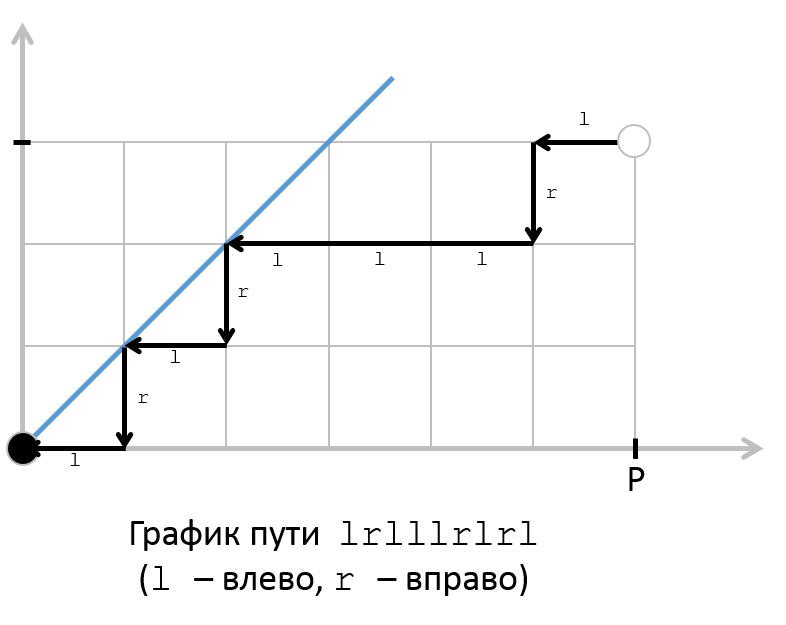
\includegraphics[width=0.5\textwidth]{figures/path1.png}
	\end{center}

	Нам нужно вычесть число графиков, которые соответствуют путям частицы, выходящим <<в канаву>>~-- то есть, за левую границу 0. Назовем такие пути <<неправильными>>. Разность $x-y$ координат точки на плоскости равна расстоянию от блуждающей частицы до нуля, стало быть, график <<правильного>> пути не содержит точек строго выше прямой $y=x$.

	Сместим график произвольного пути на клетку вниз~-- получим график $(P, Q-1)\rightarrow (0, -1)$. Теперь график <<правильного пути>> вообще не пересекает прямую $y=x$, а <<неправильного>>~-- имеет общую точку. Для неправильного пути обозначим $A$~-- первую точку его касания с прямой $y=x$ (считая от $(0, 0)$). Отразив сегмент графика $A \rightarrow (0, -1)$ относительно $y=x$, получим график $(P, Q-1) \rightarrow (-1, 0)$, который пересекает прямую $y=x$. Таким образом, мы иньективно сопоставили <<неправильный график>> $(P, Q-1)\rightarrow (0, -1)$ какому-то графику $(P, Q-1) \rightarrow (-1, 0)$. Пример <<перестройки>> графика:

	\begin{center}
		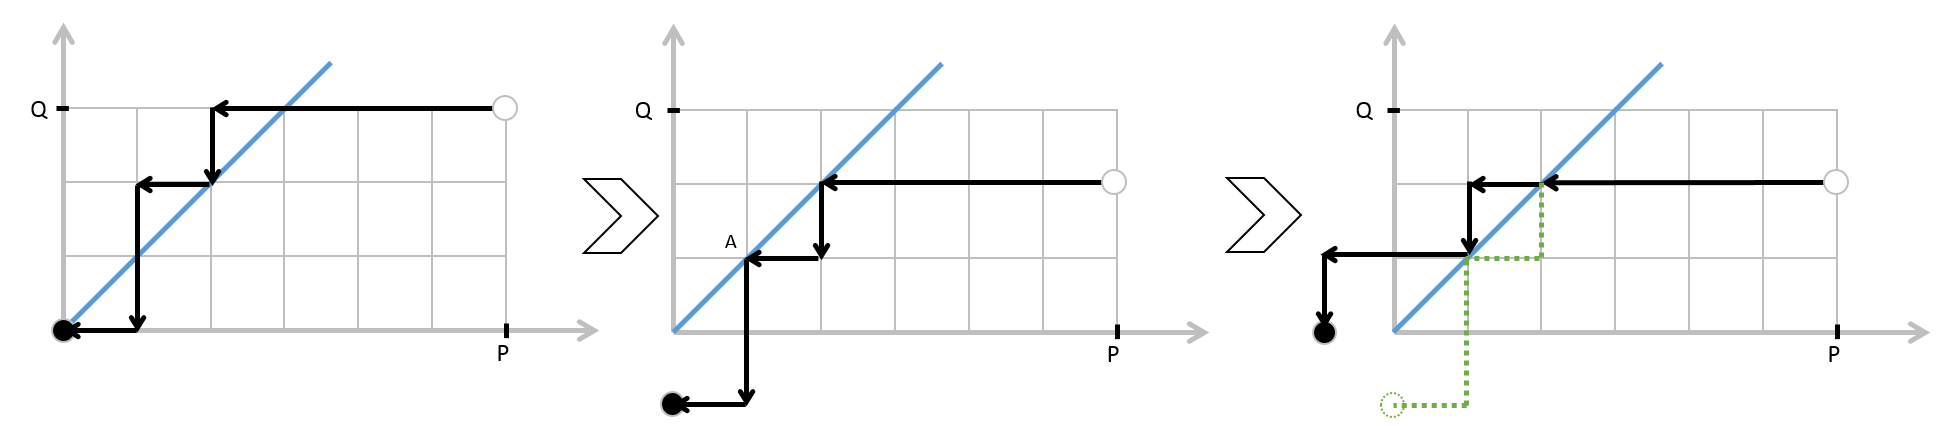
\includegraphics[width=\textwidth]{figures/path2.png}
	\end{center}

	Оказывается, это сопоставление~-- биекция. Действительно, так как любой график \\$(P, Q-1) \rightarrow (-1, 0)$ пересекает прямую $y=x$, то можно снова выделить точку пересечения и иньективно перевести график обратно в график неправильного пути $(P, Q-1) \rightarrow (0, -1)$.

	Всего путей $(P, Q-1) \rightarrow (-1, 0)$ ровно ${(P+1)+(Q-1) \choose P-1} = {P+Q\choose P-1}$, по биекции столько же <<неправильных>> графиков.

	Ответ на задачу: ${P+Q\choose P} - {P+Q\choose P-1} = \frac{P-Q}{P+Q}{P+Q\choose P}.$
\end{proof}

В нашем случае количество шагов влево $P = 2n/3$, вправо $Q=n/3$, так что всего таких путей $\frac{1}{3}{n\choose n/3}$. Для фиксированного пути с $P$ шагами влево и $Q$ шагами вправо вероятность, что $x$ пройдет именно его, равна $(1/3)^P (2/3)^Q = (1/3)^{2n/3} (2/3)^{n/3}$, так что:

$$P_2 = \frac{1}{3} {n\choose n/3} (1/3)^{2n/3} (2/3)^{n/3}$$

\newcommand{\scm}{\overset{\text{c}}{\sim}}
Символом $\scm$ будем обозначать <<эквивалентность с точностью до константы>>, т.е: $$[f \scm g] \iff [\exists C > 0: \; f \sim Cg]$$

С помощью формулы Стирлинга $n! \sim \sqrt{2\pi n}\left(\frac{n}{e}\right)^n \scm \sqrt{n}\left(\frac{n}{e}\right)^n$ можно убедиться, что:

$$ P_1 \scm \frac{1}{\sqrt n}\left(\frac{3}{2^{5/3}}\right)^n$$
$$ P_2 \scm \frac{1}{\sqrt n}\left(\frac{1}{2^{1/3}}\right)^n$$

И поэтому вероятность успеха асимптотически хотя бы
$$P \geq P_1 \cdot P_2 \scm \frac{1}{\sqrt n}\left(\frac{3}{2^{5/3}}\right)^n \cdot \frac{1}{\sqrt n}\left(\frac{1}{2^{1/3}}\right)^n = \frac{1}{n}\left(\frac{3}{4}\right)^n$$

Однако этот алгоритм работает за $O(n)$ времени! Его можно повторить много раз, увеличивая шансы на успех. В частности, если повторить его $n\left(\frac{4}{3}\right)^n = L$ раз, то имеем вероятность неудачи:

$$\left(1-\frac{1}{L}\right)^L \leq \frac{1}{e} \leq \frac{1}{2}$$

Что и приводит нас к требуемому результату.
\end{proof}

\begin{nb*}А если повторить в $q$ раз больше, то есть $qn\left(\frac{4}{3}\right)^n$ раз, то вероятность неудачи $\leq\left(\frac{1}{2}\right)^q$ можно выбрать сколь нужно малой.
\end{nb*}
